\begin{exo}{}
	On considère le tableau de variations d'une fonction $f$.

	\vspace*{2mm}
	\begin{center}
		\begin{tikzpicture}
			\tikzset{arrow style/.style={->, >=Triangle, thick}}
			\tikzset{double style/.style={double, line width=1pt, double distance=2pt, draw=black}}
			\tkzTabInit[lgt=1, espcl=1.5]{$x$ / 0.7 , $f$ / 1.3}{$-\infty$, $-2$, $1$, $5$}
			\tkzTabVar{-/ , +/ $5$, -/ $3$, +/ $4$}
		\end{tikzpicture}
	\end{center}

	\begin{enumerate}
		\item Préciser l'ensemble de définition $\mathcal{D}$ de $f$.
		\item En utilisant les termes « croissante » et « décroissante », décrire les variations de $f$.
		\item Peut-on affirmer que :
		      \begin{enumerate}
			      \item $5$ est le maximum de $f$ sur $\mathcal{D}$ ?
			      \item $3$ est le minimum de $f$ sur $\mathcal{D}$ ?
		      \end{enumerate}
	\end{enumerate}
\end{exo}
